\chapter{Overview of medical imaging}
In this chapter we are going to present a brief overview of medical imaging. First we explore the history of this field, from the 1960s to the current state. Since the aim of this work is detection and classification, we provide a review of approaches to classification task. Lastly, for better understanding of our work and the data we are working with, brief survey of computed tomography is introduced.

Medical imaging, also referred to as radiology, is the medical field which includes the production, as well as analysis and processing of medical image data \cite{diagnostic50years}. Medical professionals use methods of medical imaging, such as computed tomography (CT), magnetic resonance (MRI) or ultrasound, to depict various body parts for diagnostic purposes. With the arrival of digital era it became possible to scan and store significant amounts of medical images digitally. Over the last few decades, researchers have implemented systems to automate the analysis of medical images and it has become one of the main research subjects in the medical imaging field. 

\section{Computer-aided diagnosis}
Initially used approaches in the 1960s resided in construction of rule-based systems, which were able to solve only specific tasks \cite{surveyOnImageing}. These automated computer diagnosis systems brought the very concept of automated diagnostics. It was assumed, that they could potentially completely replace radiologists, believing that computers can achieve better performance at specific tasks, lacking the human-like disposition to making errors. However, with this goal, meeting the expectations on specificity and sensitivity of the systems was simply unattainable, since it required huge amounts of computational power, which was hard to ensure at that time. Thus, in the 1980s the direction of the medical imaging evolution was changed and another approach was presented - computer aided diagnosis (CAD) \cite{diagnostic50years}. The essence of CAD is to improve diagnostic accuracy by assisting radiologists and act as a "second opinion" \cite{surveyOnImageing, CADinmedicalImaging} to their own medical opinion. 
The progress of technology and easier access to high-performance hardware components such as central processing units (CPU) and graphics processing units (GPU) at the end of 1990s resulted in supervised machine learning systems becoming very popular in CAD \cite{surveyOnImageing}. This was viable also due to increasing amount of available medical data (big data), making it possible to train such systems. It was a big step, shifting from completely human designed systems, to ones based on manual feature extraction and then trained automatically by computers. Feature extraction lies at the heart of a successful medical image analysis, therefore the next course of action was to apply machine learning in a self-taught manner for this task as well. We provide more detailed review on deep learning in chapter 4.

% https://ieeexplore.ieee.org/abstract/document/7404017
% http://www.bioscience.org/2019/v24/af/4725/fulltext.php?bframe=2.htm
% https://link.springer.com/article/10.1007%2Fs12194-017-0406-5
% https://www.researchgate.net/profile/Niall_O_Mahony/publication/331586553_Deep_Learning_vs_Traditional_Computer_Vision/links/5cc8bfac4585156cd7bdb5ac/Deep-Learning-vs-Traditional-Computer-Vision.pdf
% https://www.sciencedirect.com/science/article/pii/S093938891830120X
% https://europepmc.org/article/med/28301734#R1
% https://ieeexplore.ieee.org/abstract/document/8241753
% https://www.ncbi.nlm.nih.gov/pmc/articles/PMC1955762/
% https://iopscience.iop.org/article/10.1088/0031-9155/51/13/R02/meta


\section{Computed tomography}
Neuroimaging is crucial when aiming for an exact diagnosis of intracranial hemorrhage.  Taking into account its wide availability and non-invasive technique, computed tomography (CT) is most commonly used in detection of intracranial hemorrhage these days \cite{imagingICH}. Even though magnetic resonance imaging (MRI) has been proven to be more sensitive, CT is able to provide much faster results, which is critical when it comes to obtaining early assessment of the presence and extent of the bleeding \cite{imagingAfterBrainInjury}. The main principle of non-contrast computed tomography imaging resides in the fact, that different tissues of the human body can absorb different amounts of X-ray beams, which is referred to as tissue density \cite{principlesOfCT}. The absorbed X-ray is being mapped into Hounsfield Units (HU). Resulting scans are formed from units of space within the patient's body called voxels. These units contain a three-dimensional (3D) information about the value of tissue density. Resulting 3D scans are studied using a method called windowing, which converts selected range of Hounsfield Units (HU) into values of grayscale (range between 0 and 255).  As a result, a two-dimensional cross sectional "slice" can be extracted from the 3D volume. The selected range is set by two different parameters: window width (WW) and window level (WL). Windowing enables radiologists to study different features and tissues by increasing the contrast, thus bringing forward the tissue of interest \cite{windowClassBiomArt}. The original CT pixel values, which are not in the selected range, are displayed either as black or white, as shown in Figure 3.1 .

\begin{figure}[h]
\begin{centering}
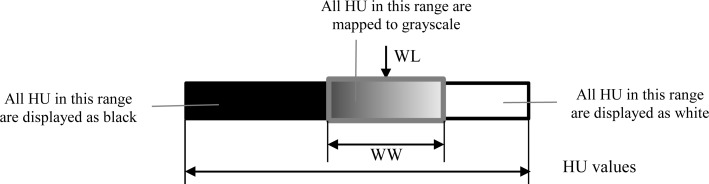
\includegraphics[width=15cm]{assets/images/windowingHU}
\par\end{centering}
\caption{Windowing of CT scans \cite{windowClassBiomArt}
\label{fig:windowing}}
\end{figure}

In detection of intracranial hemorrhage from head CT scans, blood and brain windows are the standard choice. Right after the appearance of hemorrhage, the area of the bleeding shows density values of 60 to 80 Hounsfield units (HU), and as it matures, the value increases up to 100 HU  \cite{principlesOfCT}, which can be visible in the scan slice with a correct setting of window width and window length.

\section{Deep learning in medical imaging}
\subsection{Detection}
\subsection{Classification}
\subsection{Segmentation}